\documentclass[10pt]{article}
\usepackage[utf8]{inputenc}
\usepackage[spanish, activeacute]{babel}
\usepackage{amsmath}
\usepackage{epsfig}
\usepackage{enumerate}
\usepackage{float}
\usepackage{listings}
\frenchspacing
\linespread{1.2}                                          %espacio entre líneas
\setlength{\parskip}{1.5ex plus 0.2ex minus 0.2ex}        %espacio entre párrafos
\setlength{\columnsep}{0.9cm}  				  %espacio entre columnas
\usepackage{indentfirst}
\usepackage{graphicx}
\usepackage{verbatim}
\usepackage{url}
\usepackage{multicol}
\usepackage{geometry}
\usepackage{fancyhdr}
\usepackage{moreverb}
\usepackage{hyperref}
\usepackage{acronym}

\geometry{tmargin=3.0cm, lmargin=3.0cm, rmargin=2.5cm, bmargin=3.0cm}

\newcommand\R{R}
\newenvironment{keywords}{\begin{description}\item[Palabras Claves:]}{\end{description}}
\renewcommand{\refname}{Referencias}

\title{
\center{\emph{Desarrollo de una plataforma astroinformática para la administración y análisis inteligente de datos a gran escala} \\}
\center{\textbf{Arquitectura de software - Prototipo Funcional 
	\\ Version 1.3 - 26 Diciembre} \\}
\author{Mauricio Solar, Marcelo Mendoza, Diego Mardones, Jonathan Antognini, \\ 
	Walter Fariña, Christopher Fernandez, Mario Garces, \\	
	Camilo Valenzuela, Patricio Ramirez, Marco Peña.}
\date{Valparaíso, \today}
}

\begin{document}
\maketitle

\thispagestyle{empty}

\newpage
\tableofcontents

\newpage
\section{Indice de acrónimos}
\begin{acronym}
\acro{ChiVO}{Chilean Virtual Observatory}
\acro{VO}{Virtual Observatory}
\acro{ALMA}{Atacama Large Milimiter/submilimiter Array}
\acro{UV}{Ultravioleta}
\acro{FITS}{Flexible Image Transport System}
\acro{ASDM}{ALMA Science Data Model}
\acro{J2000}{Fecha Juliana 2451545.0 Tiempo Terrestre. Es equivalente al 1 de
enero de 2000, 11:59:27.816. Se usa para indicar un instante en el tiempo
estándar para la medición de las posiciones de los cuerpos celestes y otros
eventos estelares}
\acro{B1950}{Época besseliana, es una época basada en el Año besseliano, que es
un año tropical medido en el punto donde la longitud del Sol es exactamente
280º}
\acro{Sesame}{Es un resolvedor de nombres que retorna a partir de una cadena
que representa la designación de un objeto astronómico fuera del Sistema Solar,
la posición del objeto en el cielo y otros detalles}
\acro{SIMBAD}{Base de datos que proporciona datos básicos, identificaciones
cruzadas, bibliografía y las mediciones de los objetos astronómicos fuera del
sistema solar.}
\acro{ADS}{Astrophysics Data System, es una librería/portal digital}
\acro{NED}{SA/IPAC Extragalactic Database, ofrece datos de millones de objetos
fuera de la Vía Láctea.}
\acro{IVOA}{International Virtual Observatory Alliance}
\acro{SCS}{Simple Cone Search}
\acro{SIA}{Simple Image Access}
\acro{SSA}{Simple Spectral Access}
\acro{TAP}{Table Access Protocol}
\acro{MQ}{Message Queuing}
\end{acronym}


\newpage
\section{Resumen Ejecutivo}

Ejemplo de una cita: \cite{SPECT}.


\newpage
\section{Casos de Uso ChiVO}
\noindent En la captura de requerimientos y casos de uso participaron los siguientes
astrónomos:
\begin{itemize}
	\item Diego Mardones, Universidad de Chile.
	\item Lars Nyman, Atacama Large Milimiter/submilimiter Array.
	\item Neil Nagar, Universidad de Concepción.
	\item Nelson Padilla, Pontificie Universidad Católica. 
	\item Juan de Santander, Instituto de Astrofísica de Andalucía, España.
	\item Amelia Bayo, European Southern Observatory.
\end{itemize}

\noindent El informe de requerimientos (Hito Anterior) se puede encontrar en
\cite{hrequerimientos}.

\noindent Para abordar de mejor forma los casos de uso, se mencionarán algunos
conceptos relevantes:
\begin{itemize}
	\item Los datos astronómicos en sus diferentes formatos se dividen en:
Metadata y Binarios. La metadata son datos que describen los datos de la
observación, y los binarios son los datos obtenidos de la observación.
	\item En la primera etapa el proyecto trabajará con archivos FITS.
	\item Las búsquedas en el sistema se realizan sobre la metadata. El
resultado de una búsqueda es un set de datos candidatos que coinciden con los
parámetros fijados en la búsqueda.
	\item La interacción final con el sistema es cuando el usuario decide qué
datos necesita, los selecciona y los descarga de forma local.
\end{itemize}

\subsection{Casos de Uso Generales}
Los siguientes casos de usos involucran de manera general a varios
requerimientos, por lo que se presentan en una categoría especial. 

\noindent\textbf{Caso de uso \#1}: \\
\textbf{Objetivo}: Filtrar los resultados de la búsqueda en el Portal Web. \\
\textbf{Actor}: Usuario. \\
\textbf{Necesidad}: Esencial. \\
\textbf{Prioridad}: Alta. \\
\textbf{Requerimientos Referenciados}: del 1 al 7. \\
\textbf{Descripción}: Ya que el usuario puede recibir una gran cantidad de
resultados, éste debe ser capaz de realizar un filtro sobre alguna columna de
los datos recibidos al realizar la búsqueda para así poder identificar los
datos que se encuentre buscando. Este filtro puede ser realizado en el mismo
navegador del usuario o a través de una nueva consulta. 
\vspace{1.0cm}

\noindent\textbf{Caso de uso \#2}: \\
\textbf{Objetivo}: Descargar datos desde el Portal Web. \\
\textbf{Actor}: Usuario. \\
\textbf{Necesidad}: Esencial. \\
\textbf{Prioridad}: Alta. \\
\textbf{Requerimientos Referenciados}: del 1 al 7. \\
\textbf{Descripción}: Una vez que el usuario encuentre los datos que requiere, éste procede a descargarlos. Para ello el sistema provee un enlace directo a la fuente de los datos.
\vspace{1.0cm}

\noindent\textbf{Caso de uso \#3}: \\
\textbf{Objetivo}: Visualizar una representación gráfica que compare los metadatos de los resultados de la búsqueda. \\
\textbf{Actor}: Usuario. \\
\textbf{Necesidad}: Esencial. \\
\textbf{Prioridad}:  Media. \\
\textbf{Requerimientos Referenciados}: del 1 al 7. \\
\textbf{Descripción}: Una vez que el usuario reciba un conjunto de resultados, podrá visualizarlos en gráficos acordes al tipo de búsqueda y en base a los metadatos recibidos por la búsqueda.
\vspace{1.0cm}

\noindent\textbf{Caso de uso \#4}: \\
\textbf{Objetivo}: Visualizar un producto o subproducto de los datos de la observación presente en los metadatos. \\
\textbf{Actor}: Usuario. \\
\textbf{Necesidad}: Esencial. \\
\textbf{Prioridad}: Alta. \\
\textbf{Requerimientos Referenciados}: del 1 al 7. \\
\textbf{Descripción}: Visualización de la forma geométrica de las observaciones (rectangulares o redondas); cobertura UV; Calibración de paso de banda;Espectro observado;Imagen observada en un plano del producto cuando sea posible (podría ser parte de análisis en vez de observación);
\vspace{1.0cm}

\noindent\textbf{Caso de uso \#5}: \\
\textbf{Objetivo}: Análisis de cubo FITS. \\
\textbf{Actor}: Usuario.\\
\textbf{Necesidad}: Esencial. \\
\textbf{Prioridad}: Alta. \\
\textbf{Requerimientos Referenciados}: del 1 al 7. \\
\textbf{Descripción}: Selecciona pixeles; proyección en una dimensión;flujo en un área;series de tiempo.
\vspace{1.0cm}

\noindent\textbf{Caso de uso \#6}: \\
\textbf{Objetivo}: Análisis de ASDM. \\
\textbf{Actor}: Usuario. \\
\textbf{Necesidad}: Deseable. \\
\textbf{Prioridad}: Media. \\
\textbf{Requerimientos Referenciados}: del 1 al 7. \\
\textbf{Descripción}: Selecciona voxeles; proyección en una dimensión;flujo en un área;series de tiempo.
\vspace{1.0cm}

\noindent\textbf{Caso de uso \#7}: \\
\textbf{Objetivo}: Los resultados de la búsqueda deben ser analizables para secuencias de tiempo. \\
\textbf{Actor}: Usuario. \\
\textbf{Necesidad}: Esencial. \\
\textbf{Prioridad}: Baja. \\
\textbf{Requerimientos Referenciados}: del 1 al 7. \\
\textbf{Descripción}: El usuario luego de realizar una búsqueda por tipo y/o subtipo de objeto, puede obtener los resultados de la búsqueda para ser analizados como secuencias de tiempo.
\vspace{1.0cm}

\subsection{Buscar por coordenada o región del cielo}
\noindent\textbf{Caso de uso \#8}: \\
\textbf{Objetivo}: Ingresar al Portal Web y realizar una búsqueda por coordenadas. \\
\textbf{Actor}: Usuario. \\
\textbf{Necesidad}: Esencial. \\
\textbf{Prioridad}: Alta. \\
\textbf{Requerimientos Referenciados}: 1. \\
\textbf{Descripción}: El usuario ingresa al Portal Web, rellena los campos de coordenadas y radio angular o región de cielo y realiza una búsqueda. Los parámetros de coordenada pueden pertenecer al sistema ecuatorial (J2000 o B1950), eclíptico, galáctico o supergaláctico.
\vspace{1.0cm}

\noindent\textbf{Caso de uso \#9}: \\
\textbf{Objetivo}: Realizar una búsqueda de listado de coordenadas. \\
\textbf{Actor}: Usuario. \\
\textbf{Necesidad}: Esencial. \\
\textbf{Prioridad}: Alta. \\
\textbf{Requerimientos Referenciados}: 1. \\
\textbf{Descripción}: El usuario ingresa al Portal Web, ingresa una lista de coordenadas y radios angulares o regiones de cielo y realiza una búsqueda. Los parámetros de coordenada pueden pertenecer al sistema ecuatorial (J2000 o B1950), eclíptico, galáctico o supergaláctico. También el usuario puede subir un archivo con un formato establecido por el sitio con el listado de coordenadas.
\vspace{1.0cm}

\subsection{Buscar por nombre o tipo de objeto}
\textbf{Caso de uso \#10}: \\
\noindent\textbf{Objetivo}: Ingresar al Portal Web y realizar una búsqueda por nombre en base a Sesame. \\
\textbf{Actor}: Usuario.\\
\textbf{Necesidad}: Esencial.\\
\textbf{Prioridad}: Alta.\\
\textbf{Requerimientos Referenciados}: 2. \\
\textbf{Descripción}: El usuario ingresa al Portal Web, rellena el campo de nombre según los nombres definidos en Sesame y realiza una búsqueda.
\vspace{1.0cm}

\noindent\textbf{Caso de uso \#11}: \\
\textbf{Objetivo}: Ingresar al Portal Web y realizar una búsqueda por nombre en base a catálogo de un instrumento. \\
\textbf{Actor}: Usuario.\\
\textbf{Necesidad}: Esencial.\\
\textbf{Prioridad}: Alta.\\
\textbf{Requerimientos Referenciados}: 2. \\
\textbf{Descripción}: El usuario ingresa al Portal Web, rellena el campo de nombre según los nombres definidos en Catálogos específicos de un instrumento y realiza una búsqueda.
\vspace{1.0cm}

\noindent\textbf{Caso de uso \#12}: \\
\textbf{Objetivo}: Ingresar al Portal Web y realizar una búsqueda por tipo de objeto en un área del cielo. \\
\textbf{Actor}: Usuario.\\
\textbf{Necesidad}: Esencial.\\
\textbf{Prioridad}: Alta.\\
\textbf{Requerimientos Referenciados}: 2. \\
\textbf{Descripción}: El usuario ingresa al Portal Web, rellena los campos de tipo y/o subtipos de objetos y un área del cielo y realiza una búsqueda.
\vspace{1.0cm}

\subsection{Buscar por metadatos espectrales}
\noindent\textbf{Caso de uso \#13}: \\
\textbf{Objetivo}: Ingresar al Portal Web y realizar una búsqueda espectral extragaláctica. \\
\textbf{Actor}: Usuario.\\
\textbf{Necesidad}: Esencial.\\
\textbf{Prioridad}: Alta.\\
\textbf{Requerimientos Referenciados}: 3. \\
\textbf{Descripción}: El usuario ingresa al Portal Web, rellena los campos de banda o rango de frecuencia;  y/o líneas espectrales y corrimiento al rojo (z); y/o resolución espectral y/o ruido y realiza una búsqueda.
\vspace{1.0cm}

\noindent\textbf{Caso de uso \#14}: \\
\textbf{Objetivo}: Ingresar al Portal Web y realizar una búsqueda espectral galáctica. \\
\textbf{Actor}: Usuario.\\
\textbf{Necesidad}: Esencial.\\
\textbf{Prioridad}: Alta.\\
\textbf{Requerimientos Referenciados}: 3. \\
\textbf{Descripción}: El usuario ingresa al Portal Web, rellena los campos de banda o rango de frecuencia;  y/o líneas espectrales y velocidad radial (v\_r); y/o resolución espectral y/o ruido y realiza una búsqueda.  Línea espectral incluye campos de moléculas, transición de moléculas (vibracional, rotacional o electrónica) o frecuencia en reposo de la línea espectral.
\vspace{1.0cm}

\noindent\textbf{Caso de uso \#15}: \\
\textbf{Objetivo}: Realizar una búsqueda de listado de frecuencias. \\
\textbf{Actor}: Usuario.\\
\textbf{Necesidad}: Esencial.\\
\textbf{Prioridad}: Alta.\\
\textbf{Requerimientos Referenciados}: 3. \\
\textbf{Descripción}: El usuario ingresa al Portal Web, ingresa una lista de frecuencias y realiza una búsqueda. También el usuario puede subir un archivo con un formato establecido por el sitio con el listado de frecuencias.
\vspace{1.0cm}

\subsection{Buscar por metadatos espaciales}
\noindent\textbf{Caso de uso \#16}: \\
\textbf{Objetivo}: Ingresar al Portal Web y realizar una búsqueda por resolución angular y/o campos de visión. \\
\textbf{Actor}: Usuario.\\
\textbf{Necesidad}: Esencial.\\
\textbf{Prioridad}: Media.\\
\textbf{Requerimientos Referenciados}: 4. \\
\textbf{Descripción}: El usuario ingresa al Portal Web, rellena los campos de resolución angular y/o campos de visión y realiza una búsqueda.
\vspace{1.0cm}

\subsection{Buscar por metadatos temporales}
\noindent\textbf{Caso de uso \#17}: \\
\textbf{Objetivo}: Ingresar al Portal Web y realizar una búsqueda relacionada con cuando fue realizada la observación. \\
\textbf{Actor}: Usuario.\\
\textbf{Necesidad}: Deseable.\\
\textbf{Prioridad}: Baja.\\
\textbf{Requerimientos Referenciados}: 5. \\
\textbf{Descripción}: El usuario ingresa al Portal Web, rellena los campos de tiempo, cantidad de observaciones de un objeto y/o el intervalo entre las observaciones y realiza la búsqueda.
\vspace{1.0cm}

\noindent\textbf{Caso de uso \#18}: \\
\textbf{Objetivo}: Ingresar al Portal Web y realizar una búsqueda relacionada con nivel de ruido, duración de la observación o tiempo de integración.\\
\textbf{Actor}: Usuario.\\
\textbf{Necesidad}: Esencial.\\
\textbf{Prioridad}: Alta.\\
\textbf{Requerimientos Referenciados}: 5. \\
\textbf{Descripción}: El usuario ingresa al Portal Web, rellena los campos de nivel de ruido, duración de la observación o tiempo de integración y realiza una búsqueda.
\vspace{1.0cm}

\subsection{Buscar por polarización}
\noindent\textbf{Caso de uso \#19}: \\
\textbf{Objetivo}: Ingresar al Portal Web y realizar una búsqueda por parámetros de Stokes. \\
\textbf{Actor}: Usuario.\\
\textbf{Necesidad}: Esencial.\\
\textbf{Prioridad}: Baja.\\
\textbf{Requerimientos Referenciados}: 6. \\
\textbf{Descripción}: El usuario ingresa al Portal Web, rellena los campos de parámetros de Stokes necesarios (I, Q, U y/o V) o de polarización izquierda o derecha y realiza la búsqueda.
\vspace{1.0cm}

\subsection{Cruzamiento de información}
\noindent\textbf{Caso de uso \#20}: \\
\textbf{Objetivo}: Buscar un objeto en múltiples fuentes de datos como archivos de los Satélites Spitzer y Herchel. \\
\textbf{Actor}: Usuario.\\
\textbf{Necesidad}: Esencial.\\
\textbf{Prioridad}: Media.\\
\textbf{Requerimientos Referenciados}: 7. \\
\textbf{Descripción}: El usuario ingresa al Portal Web, rellena los campos de nombre o código de objeto o coordenadas junto con un radio y se realiza la búsqueda. El sistema deberá realizar la búsqueda en base a ello en múltiples fuentes de información. Si se ingresa el nombre o código, se realiza una búsqueda teniendo en cuenta el margen error de cada fuente de datos.
\vspace{1.0cm}

\subsection{Simulaciones}
\noindent\textbf{Caso de uso \#21}: \\
\textbf{Objetivo}: Realiza una búsqueda de una simulación. \\
\textbf{Actor}: Usuario.\\
\textbf{Necesidad}: Deseable.\\
\textbf{Prioridad}: Baja.\\
\textbf{Requerimientos Referenciados}: 8. \\
\textbf{Descripción}: El usuario ingresa al Portal Web y realiza un búsqueda de una simulación.
\vspace{1.0cm}

\subsection{Servicios Bibliográficos}
\noindent\textbf{Caso de uso \#22}: \\
\textbf{Objetivo}: Rl realizar una búsqueda, desplegar en los resultados enlaces a información bibliográfica de SIMBAD. \\
\textbf{Actor}: Usuario.\\
\textbf{Necesidad}: Deseable.\\
\textbf{Prioridad}: Media.\\
\textbf{Requerimientos Referenciados}: 9. \\
\textbf{Descripción}: El usuario ingresa al Portal Web y al desplegarse los resultados de una búsqueda, cada resultado contiene un enlace a una búsqueda con todos los datos contenidos en SIMBAD, ADS y/o NED pertenecientes al/los objeto/s.


\newpage
\section{Arquitectura de ChiVO}

ChiVO es un observatorio virtual en construcción, el cual alojará datos de los
observatorios localizados en Chile, ciñéndose a los estándares de
interoperabilidad de la alianza internacional de observatorios virtuales (IVOA),
y utilizando tecnologías de última generación. Esta sección, detalla el
proceso de diseño realizado para esta iniciativa.

%Que es IVOA?
La misión de IVOA es facilitar la coordinación y colaboración necesaria para
facilitar el acceso global e integrado a los datos recogidos por los
observatorios astronómicos internacionales. Esta organización fue formada en
Junio del 2002 y tiene actualmente 21 miembros activos. Su método de trabajo es
en base a Working Groups, los cuales están a cargo de estabelcer protocolos y
estándares que describen la arquitectura general de un VO \ref{fig:ivoavacio}.
A grandes rasgos, la arquitectura posee tres capas:
\begin{itemize}
    \item Usuarios: astrónomos y científicos en general interesados por los
    datos publicados por los observatorios.
    \item Recursos: observatorios y centros que producen datos astronómicos
    (reales o simulados).
    \item Capa intermedia: esta capa define lo que es un observatorio virtual,
    es decir, de qué manera se comunican los usuarios y recursos usando
    protocolos y estándares para buscar y acceder datos.
\end{itemize}

%Arquitectura de IVOA Vacía
\begin{figure}[ht]
    \centering
    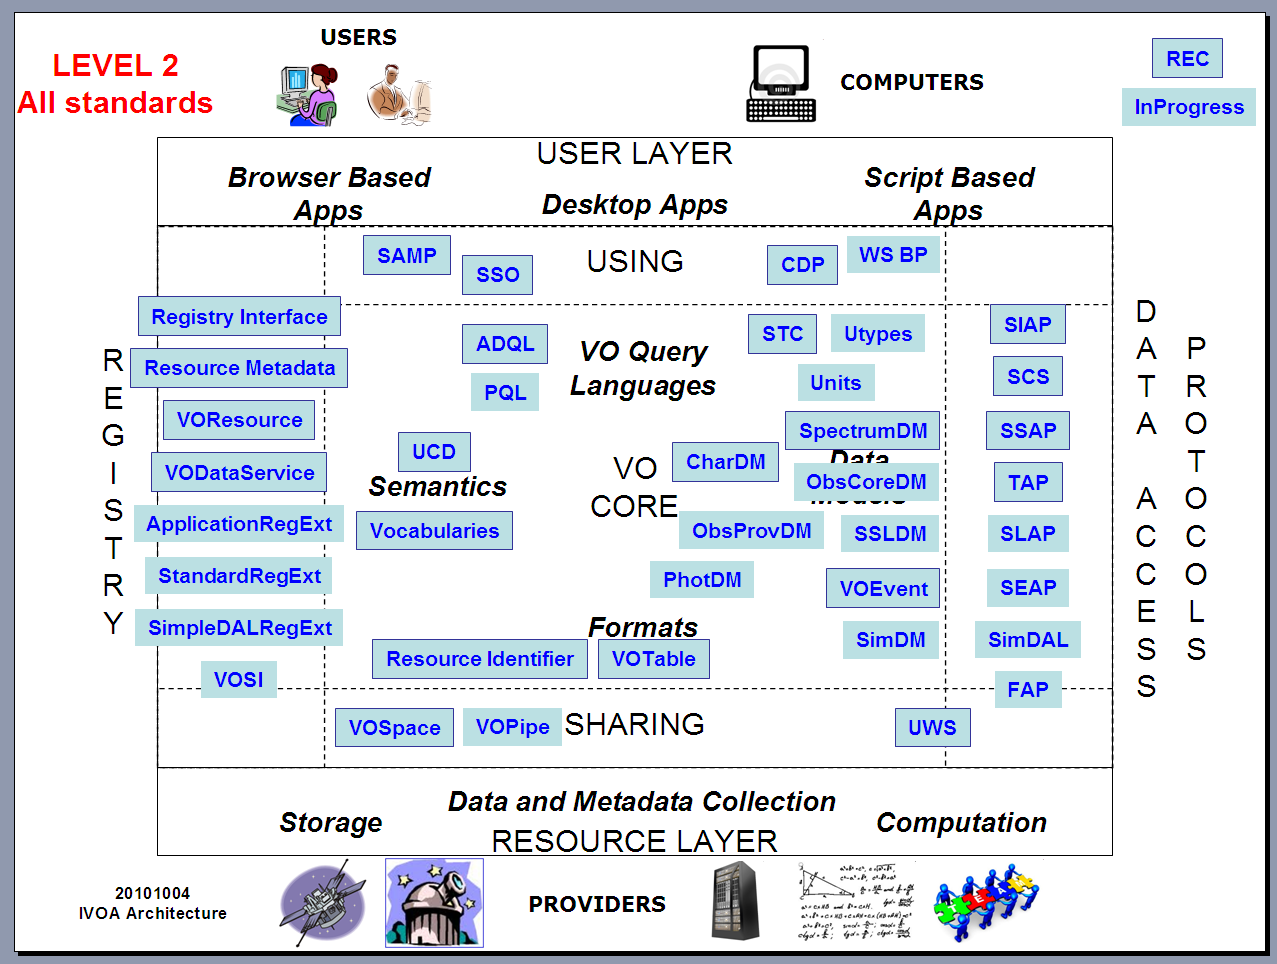
\includegraphics[width=0.45\textwidth]{images/ivoavacio.png}
    \caption{Arquitectura IVOA}
    \label{fig:ivoavacio}
\end{figure}

\subsection{Requerimientos}

Para la creación del ChiVO se identificaron las necesidades actuales de la
comunidad astronómica nacional, las cuales podemos resumir en,

\begin{description}
    \item[Descubrir:] \hfill \\
        Encontrar datos astronómicos de un objeto o instrumento sobre una región
        específica del espacio de alta dimensión, en base a parámetros de los ejes
        espaciales, temporales, espectrales, corrimiento al rojo, polarización, etc,
        ya sea por búsqueda o por exploración.
    \item[Obtener:] \hfill \\
        Enlace a descarga de los datos requeridos en distintos formatos, ya sea en
        el VO o en un servicio externo.
    \item[Comparar:] \hfill \\
        Cruzamiento de información de datos obtenidos entre distintas fuentes de
        información.
\end{description}

En este proceso participó un equipo multidisciplinario (astrónomos, ingenieros,
científicos, expertos en datos de ALMA, etc) y duró aproximadamente 4 meses,
entre que la comunidad astronómica definía bien sus requerimientos y casos de
uso, y entre que el equipo informático contrastaba estos con las normativas
internacionales.

%\textbf{TODO: poner los req?}
%[MA] NO!
%\textbf{Arquitectura IVOA}

\subsection{Arquitectura de ChiVO}

Según las necesidades de los radioastrónomos Chilenos, los requerimientos,
casos de uso y los modelos de datos (compatibles con los estándares de IVOA),
conllevan a la creación de la siguiente arquitectura y modelo de desarrollo
(ver Figura~\ref{fig:chivoarch}).

\begin{figure}[ht]
    \centering
    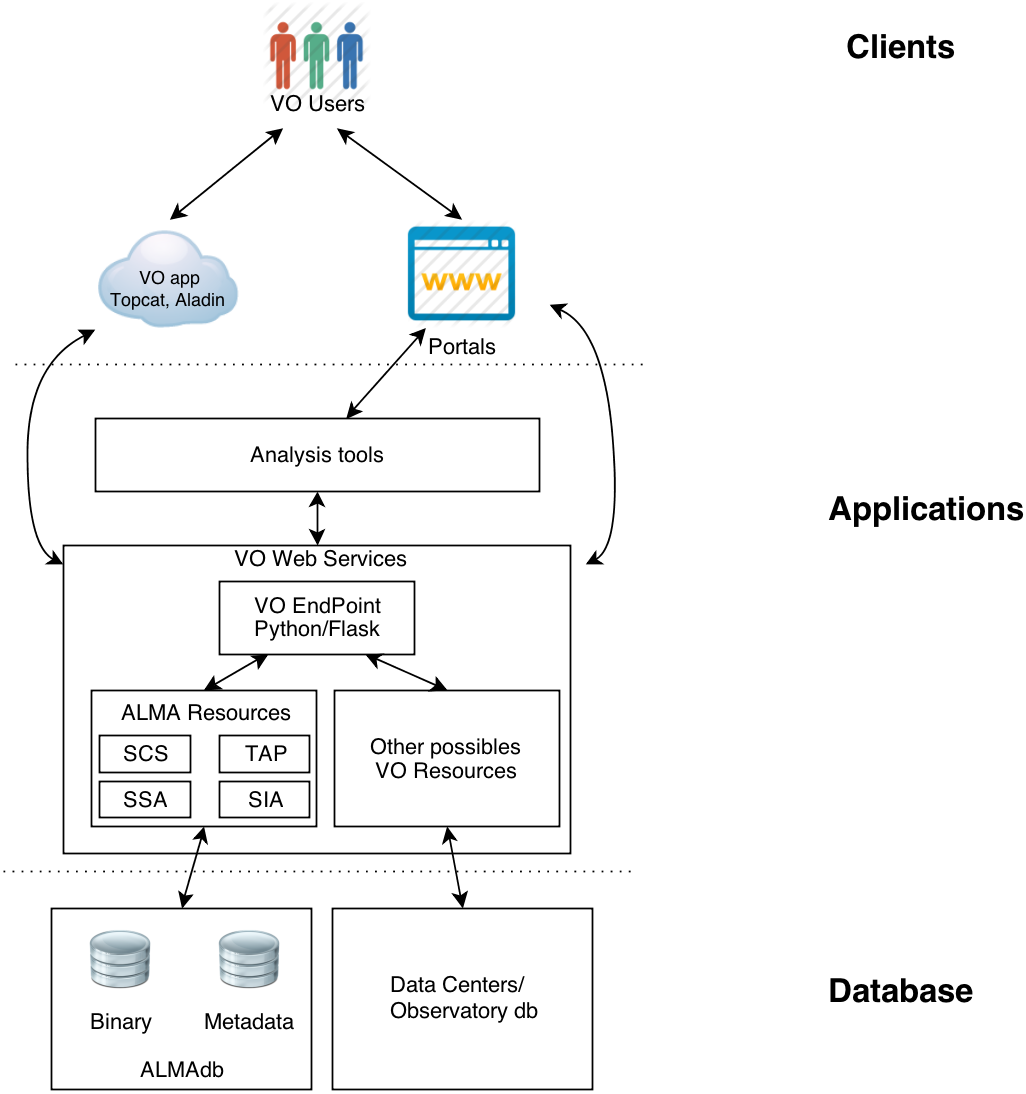
\includegraphics[width=0.45\textwidth]{images/chivo_capas.png}
    \caption{Arquitectura de ChiVO}
    \label{fig:chivoarch}
\end{figure}

\textbf{Capa de abstración: Clientes}

Esta capa representa al usuario final y cómo se facilita la comunicación entre el
usuario y los datos.  En esta capa el usuario realiza consultas a través de los
protocolos de acceso ofrecidos por ChiVO o a través de un formulario avanzado,
utilizando aplicaciones compatibles con VO y su portal web.  Una vez realizada
la consulta, el sistema le retornará al usuario una lista que describe objetos
u observaciones encontrados (metadatos) y podrá acceder a ellos a través de un
enlace de descarga asociado a cada resultado.  Cabe destacar que gracias a la
separación por capas de abstracción se logra la flexibilidad y escalabilidad en
el sistema, para que independientemente de la capa, nuevas aplicaciones puedan
interactuar con ChiVO, así como la adición de nuevas fuentes de información a
parte de ALMA.

Las consultas son recibidas por ChiVO a través de su \emph{endpoint} de datos, que
recibe consultas en \texttt{HTTP}, \texttt{GET} o \texttt{POST}, ante lo cual el
endpoint retorna la lista de resultados en una tabla en el formato XML VOTable 
\cite{ochsenbein2011ivoa}.
Para el caso del portal web, el VOTable es desplegado mostrado al usuario a través
de una herramienta web que permite la manipulación simple y eficiente de VOTables
llamada VOView.

\textbf{Capa de abstracción: Aplicaciones}

En esta capa se encuentran los programas que procesan las consultas entre los
usuarios y los datos.
Cada estándar de IVOA requiere un mínimo de su propia implementación para ser
compatible con el VO, en el caso de estos protocolos de acceso sólo es necesaria la
recepción de consultas HTTP básicas junto a los parámetros de búsqueda requeridos.

El elemento que representa a las herramientas de análisis es fundamental en la
eficiencia de ChiVO, esto es debido a que los datos a analizar por los astrónomos
suelen tener un gran tamaño y es costosa su transferencia, este problema se
resuelve acercando las herramientas de análisis y procesamiento al lugar donde están
almacenados los datos a procesar.

Considerando que en el futuro será necesario ofrecer búsquedas
basadas en otros datos, no sólo provenientes de ALMA, es necesaria cierta
abstracción al momento de implementar esta capa, ya que debe permitir la interacción
nuevas fuentes de información, siempre y cuando se mantenga la compatibilidad
de IVOA.

En esta capa también está en desarrollo un sistema capaz de resolver nombres
(tipo Sesame \cite{sesame} pero para datos de ALMA) y el registro de ChiVO.

\textbf{Capa de abstracción: Datos}

En esta capa se encuentran los recursos que tienen los datos y metadatos.  El
trabajo está asociado a una base de datos relacional para almacenar los
metadatos asociados al modelo de datos recomendado por \emph{IVOA Observation
Core Data Model} \cite{louys2011ivoa}, usando un framework desarrollado por el
VO Alemán DaCHS \cite{dachs}.  Con respecto a rendimiento, nos encontramos en
la sección que consume más recursos, tanto en tiempo de computación (resuelve
las consultas hechas a las base de datos) y además el almacenamiento físico de
los datos.  A modo de verificación momentánea, la actual implementación trabaja
con un conjunto de datos, con un tamaño de 1 TeraByte, los que provienen de la
reducción del ciclo 0 de ALMA.  Debido a esta limitación se propone el esquema
de funcionamiento de la figura \ref{fig:dachs}, en donde pueden haber N
servidores con DaCHS apuntando a M base de datos distribuidas o replicadas.

\begin{figure}[ht]
    \centering
    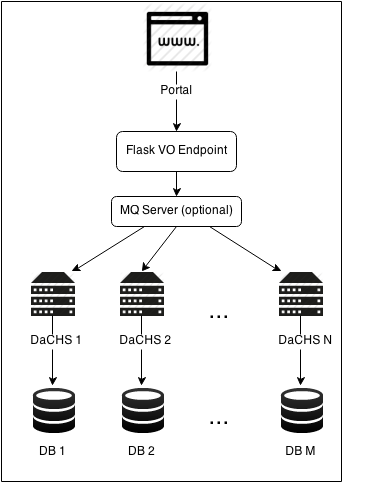
\includegraphics[width=0.45\textwidth]{images/interaccion.png}
    \caption{Configuración de distintas máquinas con base de datos replicadas o distribuidas}
    \label{fig:dachs}
\end{figure}

\subsection{Metadatos de los datos de ALMA}

Para poder construir la base de datos relacional con el modelo de datos ObsCore
fue necesario mapear campos desde el ALMA Science Data Model (ASDM)
\cite{viallefond2009sdm}.  Un ASDM contiene una serie de tablas (XML) con la
metadata de la observación, y en este caso se usaron: \emph{main},
\emph{Source}, \emph{ExecBlock}, \emph{spectralWindow}.

\begin{table}[ht]
    \centering
    \captionof{table}{Campos del ObsCore y origen desde ASDM}
    \begin{tabular}{lr}
        \textbf{Campo ObsCore} & \textbf{ASDM} \\
        dataproduct\_type      & visibility \\
        calib\_level           & 1 \\
        obs\_collection        & ALMA \\
        obs\_id                & [ExecBlock.execBlockUID] \\
        obs\_publisher\_did    & [Cycle ID] \\
        access\_url            & [URL de ChiVO] \\
        access\_format         & application/x-asdm \\
        access\_estsize        & [main.dataSize] \\
        target\_name           & [Source.sourceName] \\
        s\_ra                  & [Source.direction] \\
        s\_dec                 & [Source.direction] \\
        s\_fov                 & [1.2 * lambda / Diametro antena] \\
        s\_region              & circle \\
        s\_resolution          & [1.2*lambda/(ExecBlock.baseRangeMax)] \\
        t\_min                 & [ExecBlock.startTime] \\
        t\_max                 & [ExecBlock.endTime] \\
        t\_exptime             & [main.interval] \\
        t\_resolution          & [mainTable.interval] \\
        em\_min                & [ExecBlock.baseRangeMin] \\
        em\_max                & [ExecBlock.baseRangeMax] \\
        em\_res\_power         & [spectralWindow.resolution] \\
        o\_ucd                 & em.mm \\
        pol\_states            & [Source.stokesParameter[numStokes]] \\
        facility\_name         & ALMA \\
        instrument\_name       & ALMA \\
    \end{tabular}
    \label{table:obsasdm}
\end{table}

En la Tabla \ref{table:obsasdm} se muestra el resultado de la investigación,
a la izquierda se despliegan las columnas de la clase Observation,
la segunda columna indica de donde se obtienen los datos para asignar la los campos
de la primera columna para el caso de los ASDM.

Para poder llenar los campos de la clase Observation es necesario escribir una
rutina capaz de operar sobre las tablas del ASDM (XML).
Actualmente existen múltiples herramientas en el Paquete de Aplicaciones de Software
Comunes de Astronomía (CASA, debido a sus siglas en inglés) \cite{petry2012analysing}.

\subsection{Tecnologías utilizadas}

Para el desarrollo de ChiVO se evaluaron distintas herramientas posibles de las
cuales se concluyó en cada capa:

\textbf{Capa de abstración: Aplicación}

Los framework que se evaluaron para la implementación del endpoint fueron:

\begin{description}
    \item[{\ror}:] \hfill \\
        Framework de desarrollo web ampliamente utilizado el día de hoy,
        se basa en el concepto Modelo-Vista-Controlador (MVC).
        Sin embargo, ésta herramienta no será utilizada debido
        a que muchas funcionalidades no son necesarias para el presente prototipo.
    \item[Python/Flask:] \hfill \\
        Flask es un microframework diseñado especialmente para servicios y
        herramientas web pequeñas.
        La presente solución provee un marco de trabajo para la creación de
        aplicaciones web que puedan ser accedidas mediante distintos métodos
        HTTP.  Existe mucha documentación y comunidad activa que permite
        implementar y solucionar problemas de forma rápida.
\end{description}

\textbf{Capa de abstración: Datos}

Dentro de los \emph{toolkits} de Data Access Layer recomendados por IVOA para
el acceso a datos mediante protocolos: Simple Cone Search (SCS)
\cite{williams2008simple}; Simple Image Access (SIA) \cite{tody2004simple};
Simple Spectral Access (SSA) \cite{tody2008simple}; y Table Access Protocol
(TAP) \cite{dowler2010table} a través de Astronomical Data Query Language (ADQL)
\cite{yasuda2004astronomical} y Universarl Worker Service
\cite{rixon2008universal}, se probaron y verificaron los siguientes:

\begin{description}
    \item[SAADA:] \hfill \\
        Desarrollado por el VO Francés, es una herramienta bastante útil del punto
        de vista del usuario del sistema.
        Posee excelente documentación y un conveniente proceso de instalación.
        Está desarrollado en Java y su correspondiente despliegue se lleva a cabo
        mediante Tomcat.
        Es posible configurar servicios SCS/SIA/SSA/TAP y no es un proyecto
        OpenSource.

    \item[VO-Dance:] \hfill \\
        Desarrollado por el VO Italiano, es una herramienta en Java en su Backend,
        y Python en su Frontend (Framework Django).
        Lo destacable de esta herramienta es que trabaja usando MySQL como motor de
        base de datos principal, y de acuerdo a las últimas noticias relacionadas
        a su desarrollo, podría existir un soporte para PostgreeSQL en el futuro.
        La herramienta no es OpenSource y la documentación es precaria debido
        a que aún está en desarrollo. Compatible con servicios SCS/SIA/SSA/TAP.

    \item[openCADC:] \hfill \\
        Desarrollado por el VO Canadiense, es una herramienta OpenSource escrita en
        Java, utilizada actualmente en el ALMA Science Archive.
        Este toolkit es uno de los más robustos, contiene distintos paquetes con
        servicios a ser utilizados en el webservice, sin embargo posee una
        documentación precaria, lo que es compensado por abierta comunidad de
        desarrollo. Es posible configurar servicios TAP, UWS.

    \item[DaCHS:] \hfill \\
        Desarrollado por el VO Alemán, es una herramienta OpenSource escrita en
        Python.
        Es uno de los toolkits DAL más usados por los VO, ya que posee una amplia
        documentación de instalación y configuración.
        Es posible configurar servicios SCS/SIA/SSA/TAP.
\end{description}

%\vspace{0.5cm}
\begin{table*}[ht]
\centering
\caption{Resumen de los toolkits en tabla comparativa}
\begin{tabular}{lrrrrr}
    {\bf Toolkits} & {\bf Lenguaje} & {\bf OpenSource} & {\bf Documentación} & {\bf Servicios} & {\bf Última actualización}  \\
    SAADA          & Java           & No               & Si                  & SCS/SIA/SSA/TAP & Mayo 2012     \\
    VO-Dance       & Java/Python    & No               & No                  & SCS/SIA/SSA/TAP & Dicimbre 2012 \\
    openCADC       & Java           & Si               & No                  & TAP             & ---           \\
    DaCHS          & Python         & Si               & Si                  & SCS/SIA/SSA/TAP & Junio 2013    \\
\end{tabular}
\label{table:toolkits}
\end{table*}

\textbf{Capa de abstración: Clientes}

Inicialmente la interfaz usuario o frontend poseería solo vistas, por lo que
el desarrollo podía ser en prácticamente cualquier lenguaje o framework, como por
ejemplo PHP, Django o {\ror} Sin embargo con los requerimientos de la
plataforma, especialmente el de capa de usuarios, se decidió escoger un
framework MVC que fuese lo suficientemente ágil y compatible con el resto de
servicios, {\ror}.


\newpage
\thispagestyle{empty}
\addcontentsline{toc}{section}{Bibliografía}

\nocite{*}
\bibliographystyle{plain}
\bibliography{report}

\end{document}
